\subsection{Dynamical Systems and Equilibria}\label{subsec:dynamical-systems-and-equilibria}

    A dynamical system is a set of equations describing how a collection of quantities evolves over time. This essay will work with systems of coupled ODEs:
    \[
        \dot{x} = f\left(x,y,\mu\right), \qquad \dot{y} = g\left(x,y,\mu\right),
    \]
    where $\dot{x}$ denotes the rate of change of $x$ with respect to time $\left(\frac{dx}{dt}\right)$, $\dot{y}$ denotes the rate of change of $y$ with respect to time $\left(\frac{dy}{dt}\right)$, and $\mu$ is an external parameter that can be varied, with $x$ and $y$ depending on $\mu$ as well as each other.


    A point $\left(x^*,y^*\right)$ is an equilibrium\footnote{Also known as a fixed point.} if $f(x^*,y^*,\mu)=g(x^*,y^*,\mu)=0$. Left undisturbed, a system that starts here will stay here, since its rate of change is 0. Geometrically, these points sit at the intersection of the two nullclines, $f=0$ and $g=0$ (see Figure~\ref{fig:equilibrium}), curves in the $(x,y)$ plane along which $\dot{x}$ and $\dot{y}$ vanish \parencite{strogatzNonlinearDynamics2018}. Because both $f$ and $g$ depend on $\mu$, the shape of each nullcline, and hence the number of intersections, changes as $\mu$ varies. This parameter dependence ultimately allows the system to undergo a bifurcation.

    \begin{figure}[H]
    \centering
    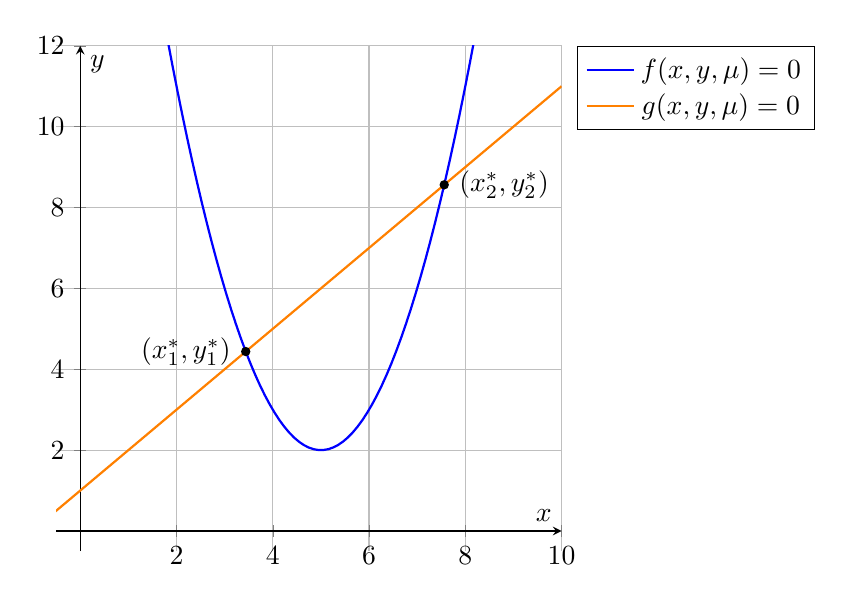
\begin{tikzpicture}
        \begin{axis}[
        width=8cm, height=8cm,
        xlabel={$x$}, ylabel={$y$},
        xmin=-0.5, xmax=10, ymin=-0.5, ymax=12,
        axis lines=middle,
        grid=both,
        legend pos=outer north east,
        ]
        \addplot[domain=0:10, blue, thick, samples=100] {(x-5)^2+2};
        \addlegendentry{$f(x,y,\mu)=0$}
        \addplot[domain=-1:10, orange, thick] {x+1};
        \addlegendentry{$g(x,y,\mu)=0$}
        \node[circle, fill=black, inner sep=1.2pt, label={left:$(x_1^*,y_1^*)$}] at (axis cs:3.438,4.438) {};
        \node[circle, fill=black, inner sep=1.2pt, label={right:$(x_2^*,y_2^*)$}] at (axis cs:7.562,8.562) {};
        \end{axis}
    \end{tikzpicture}
    \caption{Geometric representation of equilibria as intersections of the nullclines $f=0$ and $g=0$.}
    \label{fig:equilibrium}
\end{figure}


    \subsection{Energy Conservation Model}\label{subsec:energy-conservation-model}

    \[
        C\frac{dT}{dt} = Q\left[1-\alpha(T) \right]-(A+BT)
    \]

    Where...

    \begin{itemize}

        \item $C\frac{dT}{dt}$ is the rate of change of the global temperature, which is scaled by the system's effective heat capacity ($C$). In this case, the system is the planet, so a larger $C$ means more ocean, ice, etc., to warm. Thus, energy imbalances in $\frac{dT}{dt}$ will produce slower warming.

        \item $Q\left[1-\alpha(T)\right]$ is the absorbed solar radiation. $Q$ accounts for incoming solar flux and $\alpha(T)$ is the fraction reflected, known as the albedo. Thus, $1-\alpha(T)$ is the fraction absorbed by the planet.

        \item $-(A+BT)$ is the outgoing longwave radiation, which has been linearized. A hotter body radiates more, but $A+BT$ is the linear approximation for this radiation. This term was proposed in \textit{The Effect of Solar Radiation Variations on the Climate of the Earth} using observed climate data \parencite{budykoEffectSolar1969}.

    \end{itemize}
   

    \subsection{Albedo Feedback}\label{subsec:albedo-feedback}

    \[
        \alpha(T)=\frac{1}{2}\left[\left(\alpha_W+\alpha_C\right)+\left(\alpha_W-\alpha_C\right)\tanh\frac{T-T_R}{\omega}\right]
    \]
    \parencite{dortmansEnergyBalance2019}

    Where...

    \begin{itemize}

        \item $\alpha_C$ is the albedo of a fully frozen planet, which is high, as ice and snow are highly reflective

        \item $\alpha_W$ is the albedo of a fully warm planet, which is low as ocean and bare ground absorb strongly

        \item $T_R$ is a reference temperature, which is the boundary between a warm planet and a cold one

        \item $\omega$ is how fast the transition occurs

    \end{itemize}

    As $T$ increases, $\tanh\frac{T-T_R}{\omega}\rightarrow1$, so $\alpha(T)\rightarrow \alpha_W$. This means that warming reduces albedo, which increases absorbed radiation, so the planet warms faster, creating a positive feedback loop.

    \subsubsection{Expanding Terms}\label{subsubsec:expanding-terms}

    Let $u=T-T_R$.

    \[
        \tanh x = x - \frac{x^3}{3} + O(x^5) \quad\Rightarrow\quad \tanh\frac{u}{\omega} = \frac{u}{\omega} - \frac{u^3}{3\omega^3} + O\!\left(\frac{u^5}{\omega^5}\right)
    \]
    
\begin{figure}[H]
    \centering
    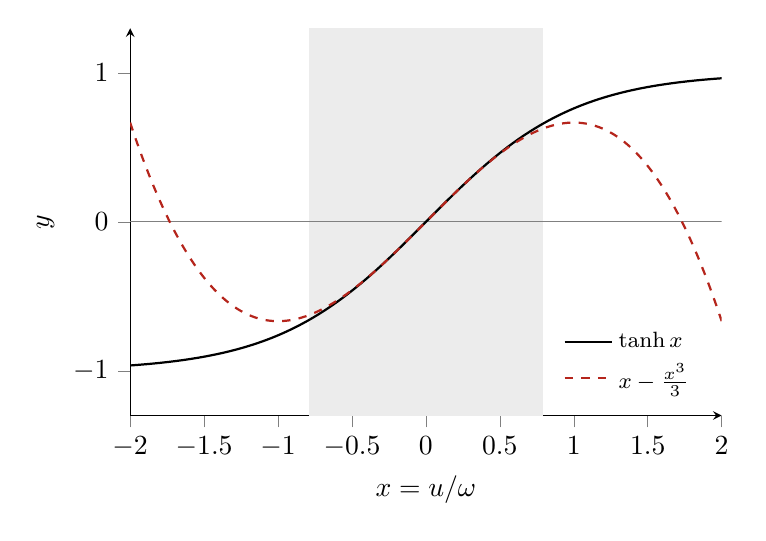
\begin{tikzpicture}
        \begin{axis}[
            width=0.75\textwidth, height=6.5cm,
            xlabel={$x=u/\omega$}, ylabel={$y$},
            xmin=-2, xmax=2, ymin=-1.3, ymax=1.3,
            axis lines=left, tick align=outside,
            legend pos=south east, legend cell align=left,
            legend style={font=\footnotesize, draw=none, fill=white, fill opacity=0.85, text opacity=1},
        ]
            \fill[gray!15] (axis cs:-0.791,-1.3) rectangle (axis cs:0.791,1.3);
            \addplot[gray, thin, forget plot] coordinates {(-2,0) (2,0)};
            \addplot[black, thick, domain=-2:2, samples=200] {tanh(x)};
            \addlegendentry{$\tanh x$}
            \addplot[BrickRed, thick, dashed, domain=-2:2, samples=200] {x - x^3/3};
            \addlegendentry{$x-\frac{x^3}{3}$}
        \end{axis}
    \end{tikzpicture}
    \caption{The Albedo function's $\tanh$ against its cubic truncation. The two agree to within 5\% in the shaded band $|x|<0.79$. When greater than $|x|=\sqrt3$, the cubic has the wrong sign}
    \label{fig:tanh-cubic}
\end{figure}

    Substituting back into $\alpha(T)$ gives:

    \[
        \alpha(T)=\frac{1}{2}\left[\left(\alpha_W+\alpha_C\right)+\left(\alpha_W-\alpha_C\right)\left(\frac{u}{\omega}-\frac{u^3}{3\omega^3}+O\left(\frac{u^5}{\omega^5}\right)\right)\right].
    \]

    Then, substituting this into the energy conservation model and substituting $T=T_R+u$:

    \[
        C\frac{dT}{dt} = Q\left[1-\frac{1}{2}\left[\left(\alpha_W+\alpha_C\right)+\left(\alpha_W-\alpha_C\right)\left(\frac{u}{\omega}-\frac{u^3}{3\omega^3}+O\left(\frac{u^5}{\omega^5}\right)\right)\right] \right]-(A+B\left(T_R+u\right)).
    \]

    Then distributing $Q$:

    \[
        C\frac{dT}{dt} = \left[Q+\left[-\frac{Q}{2}\left(\alpha_W+\alpha_C\right)-\frac{Q}{2}\left(\alpha_W-\alpha_C\right)\left(\frac{u}{\omega}-\frac{u^3}{3\omega^3}+O\left(\frac{u^5}{\omega^5}\right)\right)\right] \right]-(A+B\left(T_R+u\right)).
    \]

    \[
        C\frac{dT}{dt} = Q-\frac{Q}{2}\left(\alpha_W+\alpha_C\right) -\frac{Q\left(\alpha_W-\alpha_C\right)}{2\omega}u+\frac{Q\left(\alpha_W-\alpha_C\right)}{6\omega^3}u^3+O\left(\frac{u^5}{\omega^5}\right)-A-B\left(T_R+u\right)
    \]

    \[
        C\frac{du}{dt} = \left[Q-\frac{Q}{2}\left(\alpha_W+\alpha_C\right)-A-BT_R\right] + \left[-\frac{Q\left(\alpha_W-\alpha_C\right)}{2\omega}-B\right]u+\frac{Q\left(\alpha_W-\alpha_C\right)}{6\omega^3}u^3+O\left(\frac{u^5}{\omega^5}\right)
    \]

    For the sake of brevity, we will use the shorthand $\dot u = c_0+c_1u+c_3u^3$.

    As seen, there is no $u^2$ coefficient in this relationship because $\tanh$ is an odd function; the Maclaurin expansion only contains odd powers. Every term of the series inherits this oddness.


    \subsubsection{The Cubic Coefficient}\label{subsubsec:the-cubic-coefficient}

    A warmer planet reflects less light, so $\alpha_W<\alpha_C$. The cubic coefficient is $\frac{Q\left(\alpha_W-\alpha_C\right)}{6\omega^3}$. As $\alpha_W-\alpha_C<0$ and $Q,\omega>0$, this coefficient is negative. This means that as $|u|$ grows large, the cubic function dominates the other terms and pulls $u$ toward zero. This function stops the temperature from running away in either direction.


    \subsubsection{Rescaling}\label{subsubsec:rescaling}

    We will define $u=sT$ and $t=\tau_0\tau$, where $s$ and $\tau_0$ are currently undefined constants. Using the chain rule, $\dot u = \frac{du}{dt}=\frac{\frac{s}{\tau_0}dT}{d\tau}$. Substituting into the original equation gives:

    \[
        C\frac{s}{\tau_0}\frac{dT}{d\tau}=c_0+c_1sT+c_3s^3T^3.
    \]

    Dividing by the linear term $c_1s$:

    \[
        \frac{C}{c_1\tau_0}\frac{dT}{d\tau}=\frac{c_0}{c_1s}+T+\frac{c_3s^2}{c_1}T^3.
    \]

    Solving for $s$ such that the cubic coefficient is $-\frac{1}{3}$:

    \[
        \frac{c_3s^2}{c_1}=-\frac{1}{3}
    \]

    \[
        s=\sqrt{\frac{-c_1}{3c_3}}.
    \]

    To simplify the relationship further, we will rename the term $\frac{C}{c_1\tau_0}$ to $\epsilon$. For simplicity of future calculations, we will set $\epsilon=1.0$, working backwards solving for $\tau_0$:

    \[
        \tau_0=\frac{C}{c_1\epsilon}
    \]

    \[
        \tau_0=\frac{C}{c_1}.
    \]

    Finally, we set $\frac{c_0}{c_1s}=\mu$, which removes the physical constants and leaves dimensionless parameters. This leaves the final relationship as:

    \[
        \epsilon\dot T= T-\frac{1}{3}T^3+\mu.
    \]
    
    
        Thus far, the albedo depends only on $T$, but land ice also reflects sunlight. Following KCG, the albedo gains a term proportional to the ice extent, $\alpha(T,L)=\alpha(T)+kL$ \parencite{plociniczakHopfBifurcation2019}. This adds the term $-QkL$ to the energy-balance model; rescaling to make the coefficient of $L$ one, the temperature equation becomes $\epsilon\dot T=T-\frac{T^3}{3}-L+\mu$.

    \subsubsection{The Ice Equation}\label{subsubsec:the-ice-equation}

    \[
        \dot L = \delta(T-a)
    \]
    \parencite{kallenFreeOscillations1979}, where:

    \begin{itemize}

        \item $\dot L$ is the rate of change of ice extent.
        \item $\delta$ is the ice response rate constant, determining how fast $L$ reacts to the gap between $T$ and $a$.
        \item $a$ is the threshold temperature ($T^*=a$), and the bifurcation parameter varied in Section~\ref{sec:numerical-analysis}.
    \end{itemize}
    	The ice sheet grows when $T>a$ because a warmer climate produces more snowfall at high latitudes, and shrinks when $T<a$ because a colder and drier climate allows melting to dominate \parencite{plociniczakHopfBifurcation2019}.
    	
    \subsection{Equilibrium}
    As an equilibrium will fall when both rates are zero, we will set $\dot L =0$
    \[
    \delta(T^*-a)=0,
    \]
   as $\delta\neq0$, this gives $T^*=a$. Now setting $\dot T=0$:
   \[
   \left(T^*-\frac{T^{*3}}{3}-L^*+\mu\right)=0
   \]
   Multiplying by $\epsilon$ and substituting in $a$ gives
   \[
   L^*=a-\frac{a^3}{3}+\mu.
   \]
    
    

    \section{Linearizing \& Expanding the Cubic}\label{sec:linearizing}

    As it stands, we cannot solve the nonlinear system in closed form, but near the system's equilibrium, we can use a linear approximation with a closed-form solution. $\eta=T-T^*$ and $\xi=L-L^*$ measure the displacement from equilibrium. Starting with the derived model with $\dot T$ isolated:
    \[
        \dot{T}=\frac{1}{\epsilon}\left(T-\frac{T^3}{3}-L+\mu\right),
    \]
    We then rearrange the displacement equations to solve for $T$ and $L$:
    \[
        T=T^*+\eta
    \]
    \[
        L=L^*+\xi.
    \]
    Then, we can substitute the equilibrium values found in Section \ref{subsubsec:the-ice-equation} and expand the binomial:
    \[
        \left(T^*,L^*\right)=\left(a, \ a-\frac{a^3}{3}+\mu\right)
    \]
    \[
        \epsilon\dot \eta=(a+\eta)-\frac{(a+\eta)^3}{3}-(L^*+\xi)+\mu
    \]
    \[
        \epsilon\dot \eta=(a+\eta)-\frac{a^3+3a^2\eta+3a\eta^2+\eta^3}{3}-(L^*+\xi)+\mu
    \]
    \[
        \epsilon\dot\eta=a+\eta-\frac{a^3}{3}-a^2\eta-a\eta^2-\frac{\eta^3}{3}-(L^*+\xi)+\mu
    \]
    Now, looking at the terms with zero powers of $\eta$ and $\xi$, we know these will equal zero because:
    \[
        0=a-\frac{a^3}{3}-L^*+\mu.
    \]
    Rearranging this gives:
    \[
        L^*=a-\frac{a^3}{3}+\mu.
    \]
    This matches the expression found earlier, which confirms that the constant terms equal zero. This leaves us with:
    \[
        \epsilon\dot\eta=\eta-a^2\eta-a\eta^2-\frac{\eta^3}{3}-\xi.
    \]
    Collecting the powers and separating the linear and nonlinear parts:
    \[
        \epsilon\dot\eta=\left(1-a^2\right)\eta-\xi-a\eta^2-\frac{1}{3}\eta^3.
    \]
    Now, we will discard the nonlinear term, as this investigation only focuses on the linear approximation for small values of $\eta$ to determine at what point the approximation loses accuracy:
    \[
        \epsilon\dot\eta=\left(1-a^2\right)\eta-\xi.
    \]
    Looking at the other half of the system now:
    \[
        \dot L=\delta(T-a),
    \]
    substituting $T=a+\eta$:
    \[
        \dot L = \delta(a+\eta-a)
    \]
    \[
        \dot L = \delta\eta.
    \]
    Now, given that $\dot\xi=\dot L$:
    \[
        \dot\xi=\delta\eta.
    \]
    We can now combine these two first-order coupled differential equations into one second-order differential equation by taking the derivative of the first with respect to $t$:
    \[
        0=\left(1-a^2\right)\dot\eta-\dot\xi-\epsilon\ddot\eta.
    \]
    Substituting in for $\dot\xi$:
    \[
        0=-\delta\eta+\left(1-a^2\right)\dot\eta-\epsilon\ddot\eta.
    \]
    As this a linear second order ODE with constant coefficients we can assume $\eta=e^{\lambda t}$ ($\dot\eta=\lambda e^{\lambda t}$, $\ddot\eta=\lambda^2 e^{\lambda t}$). Substituting this into the expression:
    \[
        0=-\delta e^{\lambda t}+\left(1-a^2\right)\lambda e^{\lambda t}-\epsilon\lambda^2 e^{\lambda t}
    \]
    Dividing through by $e^{\lambda t}$ (cannot equal zero, so no solutions are lost):
    \[
        0=-\delta+\left(1-a^2\right)\lambda-\epsilon\lambda^2.
    \]
    Solving this for $\lambda$ using the quadratic formula:
    \[
        \lambda=\frac{\left(1-a^2\right)\pm\sqrt{\left(1-a^2\right)^2-4\epsilon\delta}}{2\epsilon}.
    \]
    The character of the solution depends on the sign of the discriminant, $\Delta=\left(1-a^2\right)^2-4\epsilon\delta$.

    \begin{table}[H]
        \centering
        \begin{tabular}{lll}
            \toprule
            \textbf{$\Delta$} & \textbf{Roots} & \textbf{Behavior} \\
            \midrule
            $\Delta<0$ & complex conjugate pair  & oscillation \\
            $\Delta>0$ & two distinct real roots & growth or decay \\
            $\Delta=0$ & one real root           & boundary case \\
            \bottomrule
        \end{tabular}
        \caption{Character of the Roots by Sign of the Discriminant $\Delta$}
        \label{tab:discriminant}
    \end{table}

    This essay specifically examines the case where $\Delta<0$, as that is the only case which results in oscillation. We obtain two nonreal solutions, which we can write as $\alpha\pm\beta i$. Where $\alpha=\frac{1-a^2}{2\epsilon}$ and $\beta=\sqrt{\frac{\delta}{\epsilon}-\alpha^2}$. For our numerical analysis, we will set $\delta=0.4$, as this keeps the discriminant negative as $a$ increases from 0.80 to 1.20 ($\Delta<0$ across the whole range). This means that $\lambda=0.13875\pm0.61705i$.

    \section{The Auxiliary Equation}\label{sec:auxiliary-equation}

    \subsection{General Real Solution}\label{subsec:general-real-solution}

    As it stands
    \[
        \eta(t)=Ae^{\lambda_1t}+Be^{\lambda_2t}=Ae^{(\alpha+\beta i)t}+Be^{(\alpha-\beta i)t}.
    \]
    As this function describes real-world phenomena using complex numbers, it cannot be used to predict the growth rate or period. To address this, we must separate the real part from the nonreal part:
    \[
        \eta(t)=e^{\alpha t}\left(Ae^{\beta ti}+Be^{-\beta ti}\right).
    \]
    Now that things are separated, we can apply Euler's formula to the nonreal part:
    \[
        \eta(t)=e^{\alpha t}\left(A(\cos\beta t+ i\sin\beta t)+B(\cos(-\beta t)+i\sin(-\beta t) \right).
    \]
    As sine is an odd function and cosine is an even function, we can rearrange the terms:
    \[
        \eta(t)=e^{\alpha t}(A(\cos\beta t+ i\sin\beta t)+B(\cos\beta t-i\sin\beta t)
    \]
    \[
        \eta(t)=e^{\alpha t}(A\cos\beta t+B\cos\beta t + iA\sin\beta t-iB\sin\beta t)
    \]
    \[
        \eta(t)=e^{\alpha t}(\cos(\beta t)(A+B) + \sin(\beta t)(A-B)i)
    \]
    We can define
    \[
        (A+B)=C_1
    \]
    and
    \[
        (A-B)i=C_2.
    \]
    Our final relationship is now
    \[
        \eta(t)=e^{\alpha t}(C_1\cos\beta t+C_2\sin\beta t).
    \]
    Plugging this back into the original differential equation, $0=-\delta\eta+\left(1-a^2\right)\dot\eta-\epsilon\ddot\eta$, proves our function for $\eta(t)$ to be accurate. This form of the function is valuable as it isolates the amplitude of the function, $e^{\alpha t}$, from the oscillating part of the function, $C_1\cos\beta t+C_2\sin\beta t$.

    \subsection{Interpretation of $\alpha$ and $\beta$ and $\eta(t)$ in the Real World}\label{subsec:interpretation}

    \begin{itemize}
        \item $\alpha$ is the rate of growth and decay. When $\alpha>0$, the oscillation grows. When $\alpha<0$ the oscillation shrinks towards equilibrium. Its unit is $\frac{1}{t}$
        \item $\beta$ is angular frequency, so the period of the oscillation is $P=\frac{2\pi}{\beta}$. For the parameters outlined earlier, $P=\frac{2\pi}{0.617}=10.18$ time units.
        \item $\eta(t)$ is the displacement of temperature from equilibrium.
    \end{itemize}

    \subsection{Stability}\label{subsec:stability}

    From Section~\ref{sec:linearizing},
    \[
        \alpha=\frac{1-a^2}{2\epsilon},
    \]
    and as $\epsilon>0$, the sign of $\alpha$ is determined by $1-a^2$.

    \begin{table}[H]
        \centering
        \begin{tabular}{lll}
            \toprule
            \textbf{$a$} & \textbf{$\alpha$} & \textbf{Behavior} \\
            \midrule
            $a<1$ & $\alpha>0$ & growing oscillation (unstable equilibrium) \\
            $a=1$ & $\alpha=0$ & boundary (bifurcation) \\
            $a>1$ & $\alpha<0$ & shrinking oscillation (stable equilibrium) \\
            \bottomrule
        \end{tabular}
        \caption{Stability of the Equilibrium as a Function of $a$}
        \label{tab:stability}
    \end{table}

    This justifies choosing the range $0.80\leq a\leq 1.20$, as this limited range ensures that the unique qualitative changes at $a=1$ are understood and accounted for.

    \subsection{Predictions}\label{subsec:predictions}

    The linearization of the model predicts that the oscillation period will be $\frac{2\pi}{\beta}$, which, when $a=0.85$, gives $P=10.18$, and it predicts that the amplitude of the function grows or decays at the rate $\alpha$, which, when $a=0.85$, gives $\alpha=0.139$. This is the basis for answering the research question, as these values generated from the linearization of the model can be compared using a numerical solution to the system.